\section{Experiments}

\begin{frame}
\frametitle{Experiments}
\framesubtitle{Detecting NDRAs}

\begin{table}[]
\begin{tabular}{l|cccccc}
\hline
\textbf{Sources} & \textbf{Decision} \cite{kopuklu2021driver} & \textbf{Sum} & \textbf{Conv} & \textbf{SE} & \textbf{AFF} & \textbf{MHSA (our)} \\ \hline
\textbf{Top (D)}          & 91.3 & \multicolumn{5}{c}{\textbf{92.9}}                  \\
\textbf{Top (IR)}         & 88.0 & \multicolumn{5}{c}{\textbf{91.3}}                  \\
\textbf{Top (D+IR)}       & 91.7 & 91.7 & 92.2 & 92.3 & 92.5          & \textbf{92.9} \\ \hline
\textbf{Front (D)}        & 90.0 & \multicolumn{5}{c}{\textbf{91.7}}                  \\
\textbf{Front (IR)}       & 87.0 & \multicolumn{5}{c}{\textbf{90.2}}                  \\
\textbf{Front (D+IR)}     & 92.0 & 92.7 & 92.9 & 92.9 & \textbf{93.1} & \textbf{93.1} \\ \hline
\textbf{Top+Front (D)}    & 96.1 & 94.8 & 05.8 & 05.9 & 96.5          & \textbf{96.7} \\
\textbf{Top+Front (IR)}   & 93.1 & 94.5 & 94.6 & 94.9 & 95.0          & \textbf{95.7} \\
\textbf{Top+Front (D+IR)} & 96.6 & 96.3 & 96.2 & 96.4 & 96.7          & \textbf{97.0} \\ \hline
\end{tabular}
\caption{The AUC-ROC scores of different fusion methods on the NDRAs detection task on DAD. \textbf{D} and \textbf{IR} denote the depth and infrared modalities, respectively. The best scores for each view and modality are in \textbf{bold}.}
\label{tab:1}
\end{table}

\end{frame}

\begin{frame}
\frametitle{Experiments}
\framesubtitle{Classifiying Drivers' Actions}

\begin{table}[]
\begin{tabular}{l|cccccc}
\hline
\textbf{Source}        & \textbf{Decision} & \textbf{Sum} & \textbf{Conv} & \textbf{SE} & \textbf{AFF} & \textbf{MHSA (ours)}                  \\ \hline
\textbf{Top (D)}       & \multicolumn{6}{c}{84.3}                                                                                              \\
\textbf{Top (IR)}      & \multicolumn{6}{c}{83.7}                                                                                              \\
\textbf{Top (D+IR)} &
    84.5 &
    85.0 &
    85.4 &
    85.4 &
    85.4 &
    \textbf{85.7} \\ \hline
\textbf{Front (D)}     & \multicolumn{6}{c}{87.7}                                                                                              \\
\textbf{Front (IR)}    & \multicolumn{6}{c}{83.7}                                                                                              \\
\textbf{Front (D+IR)} &
    87.9 &
    87.7 &
    88.1 &
    88.2 &
    88.5 &
    \textbf{88.7} \\ \hline
\textbf{Top+Front (D)} & 90.7              & 90.1         & 90.4          & 90.5        & 90.6         & \textbf{90.9} \\
\textbf{Top+Front (IR)} &
    88.4 &
    89.9 &
    90.2 &
    90.2 &
    90.4 &
    \textbf{90.6} \\
\textbf{Top+Front (D+IR)} &
    90.9 &
    90.8 &
    91.2 &
    91.4 &
    91.5 &
    {\textbf{91.6}} \\ \hline
\end{tabular}%
\caption{The mAP scores for multi-classification of drivers' activities on DAD.}
\label{tab:2}
\end{table}

\end{frame}

\begin{frame}
\frametitle{Experiments}
\framesubtitle{Classifiying Drivers' Actions}

{
\definecolor{myred}{HTML}{FF6666}
\definecolor{mygreen}{HTML}{00CC66}
\begin{figure}
    \centering
    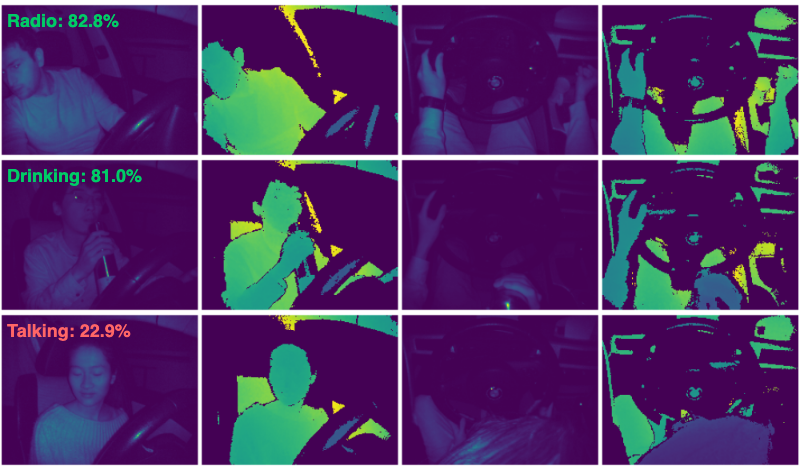
\includegraphics[width=0.72\textwidth]{images/vis.png}
    \caption{Visualisation of the middle frames of four test samples from DAD.}
    \label{fig:7}
\end{figure}
}

\end{frame}

% \begin{frame}
% \frametitle{Experiments}
% \framesubtitle{Robustness against Modality/View Collapses}

% \begin{figure}[tb]
% \centering

% \begin{subfigure}{0.49\linewidth}
%     \centering
%     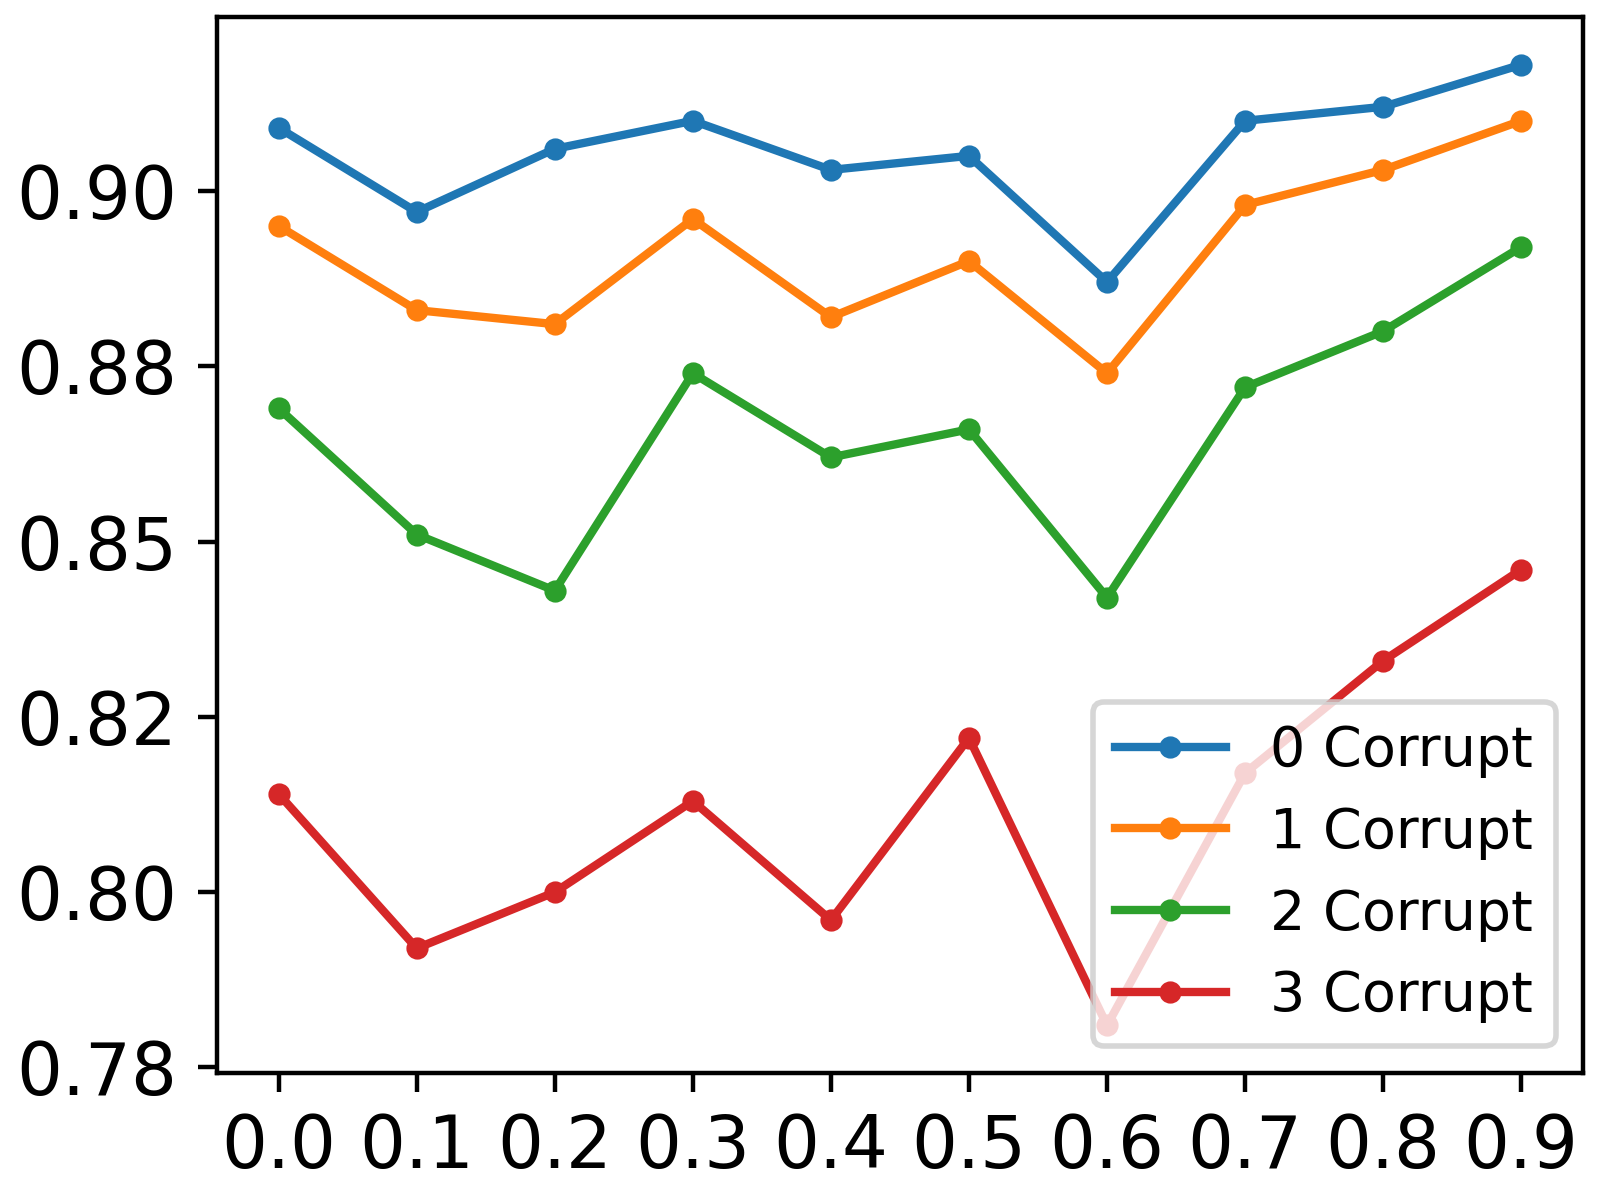
\includegraphics[width=\textwidth]{images/dtc_acc.png}
%     \caption{Det. Acc.}
%     \label{fig:robust_dtc_acc}
% \end{subfigure}
% \hfill
% \begin{subfigure}{0.49\linewidth}
%     \centering
%     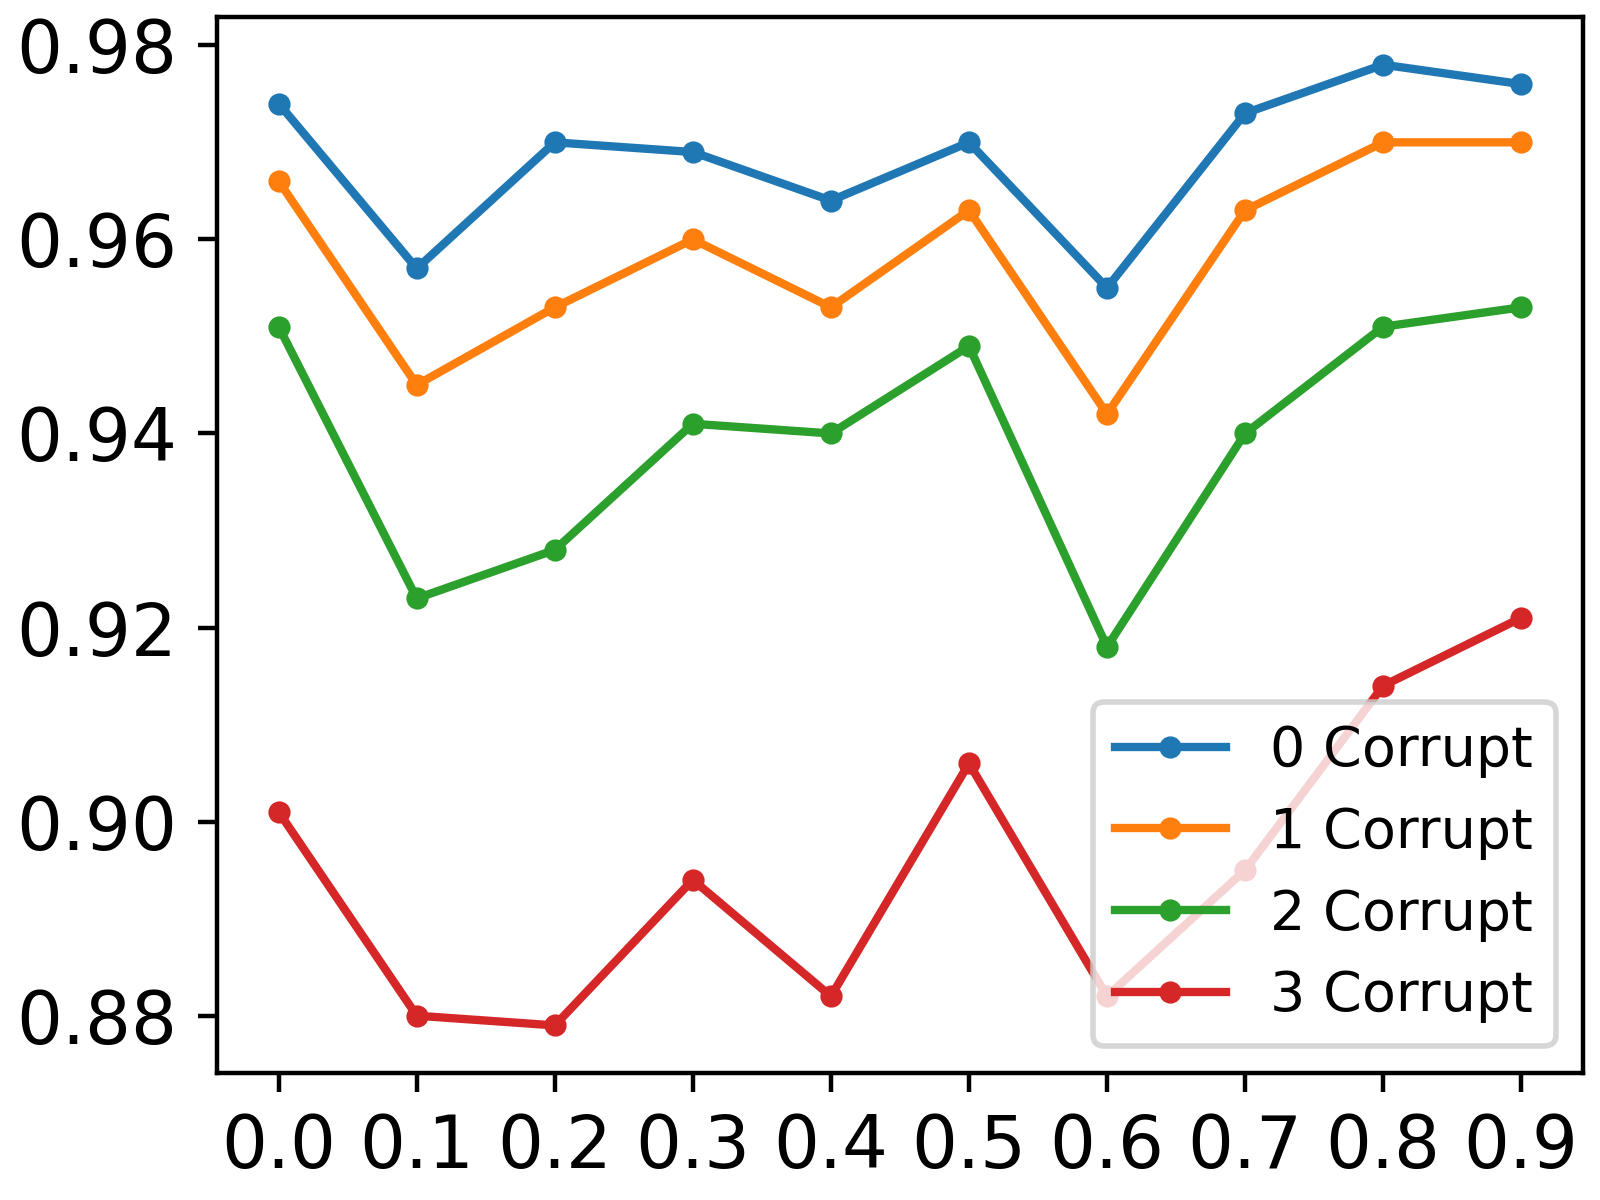
\includegraphics[width=\textwidth]{images/dtc_pr.png}
%     \caption{Det. mAP}
%     \label{fig:robust_dtc_pr}
% \end{subfigure}
% \caption{Masked training improves MHSA's robustness against corrupt views/modalities.}
% \label{fig:8}
% \end{figure}
% \end{frame}

\begin{frame}
\frametitle{Experiments}
\framesubtitle{Robustness against Modality/View Collapses}

\begin{figure}[tb]
\centering
\begin{subfigure}{0.49\linewidth}
    \centering
    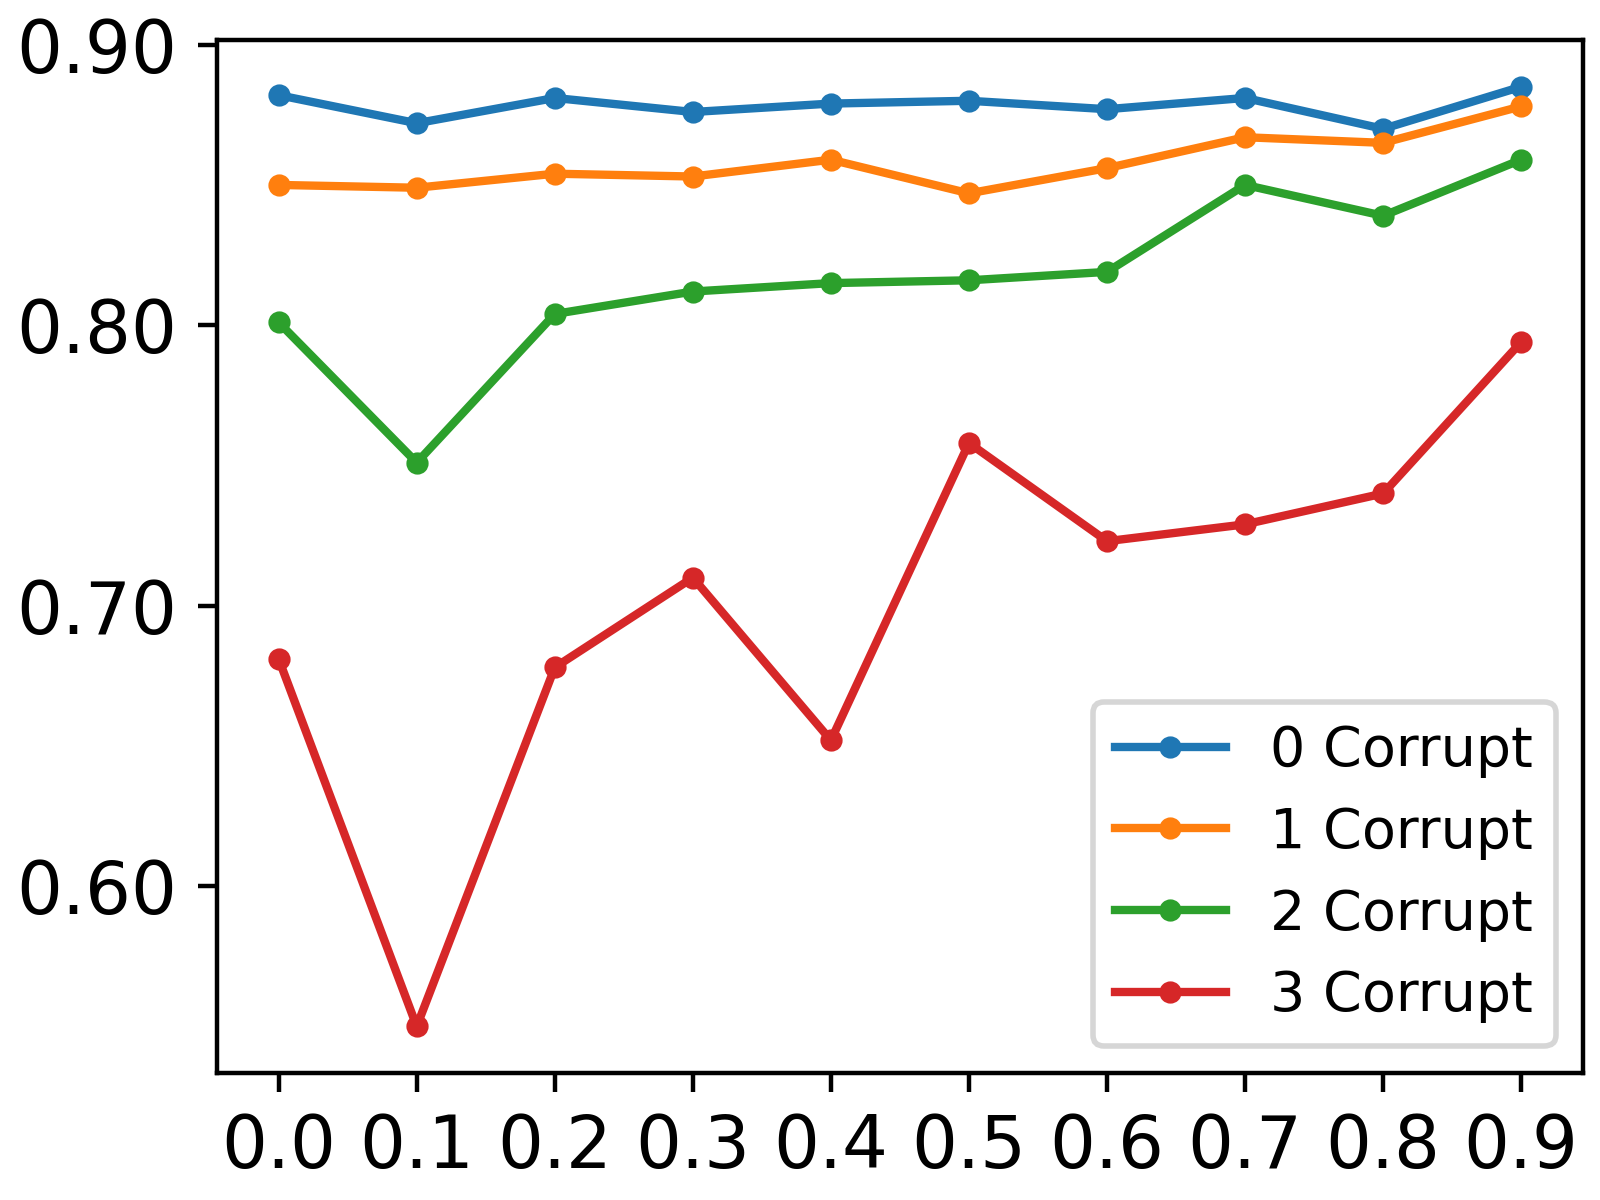
\includegraphics[width=\textwidth]{images/cls_acc.png}
    \caption{Mult. Acc.}
    \label{fig:robust_cls_acc}
\end{subfigure}
\hfill
\begin{subfigure}{0.49\linewidth}
    \centering
    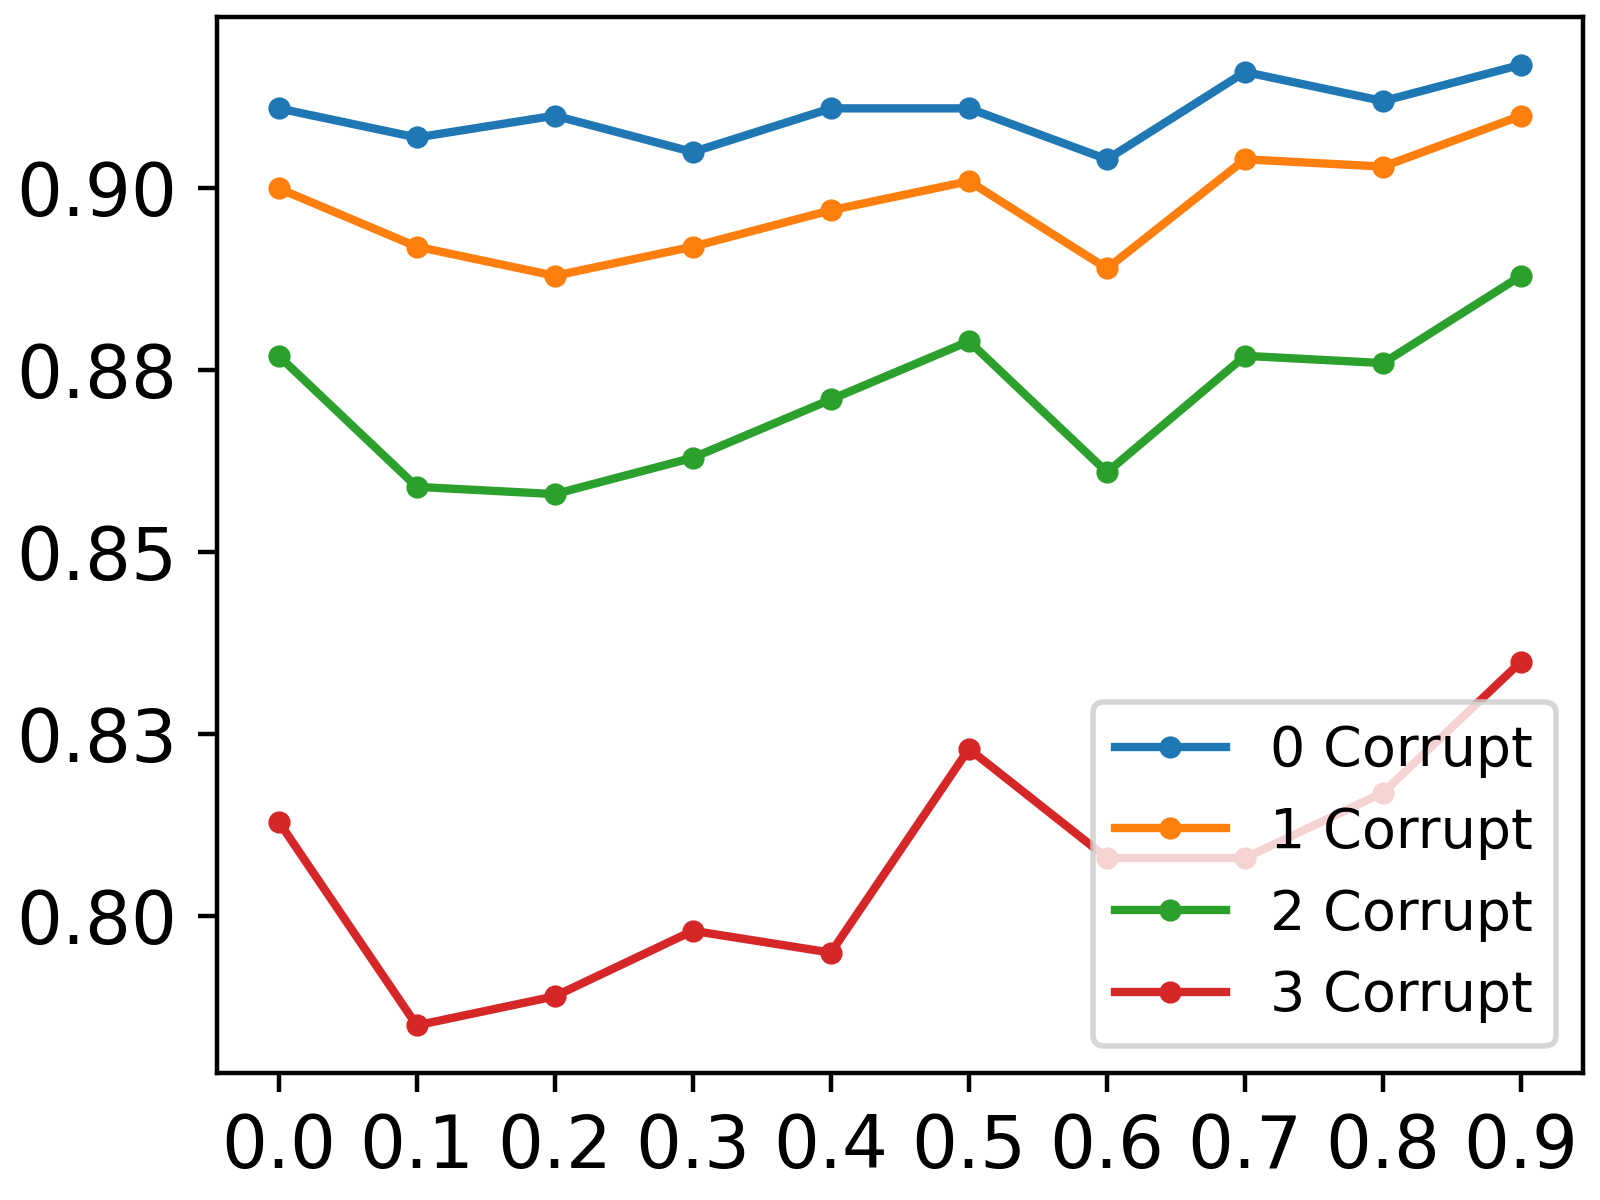
\includegraphics[width=\textwidth]{images/cls_pr.png}
    \caption{Mult. mAP}
    \label{fig:robust_cls_pr}
\end{subfigure}
\hfill
\caption{Masked training improves MHSA's robustness against corrupt views/modalities.}
\label{fig:9}
\end{figure}
\end{frame}
